\documentclass[a4paper]{article}
\usepackage[left=1cm, right=1cm, top=1cm, bottom=1cm]{geometry}
\usepackage{amsmath}
\usepackage{amssymb}
\usepackage{amsfonts}
\usepackage{subcaption}
\usepackage{caption}
\usepackage{graphicx}
\usepackage{fullpage}
\usepackage{bm}
\usepackage{xspace}
\usepackage{xcolor}
\usepackage{textcomp}

\usepackage[linesnumbered,ruled]{algorithm2e}
\makeatletter
\def\BState{\State\hskip-\ALG@thistlm}
\makeatother
\usepackage{listings}
\lstset{ 
  language=Matlab, % choose the language of the code
  basicstyle=\fontfamily{pcr}\selectfont\footnotesize\color{black},
  keywordstyle=\color{red}\bfseries, % style for keywords
  numbers=none, % where to put the line-numbers
  numberstyle=\tiny, % the size of the fonts that are used for the line-numbers
%  keywordstyle     = \bfseries,
  identifierstyle  = \color{blue},
  commentstyle     = \color{olive},     
  backgroundcolor=\color{white},
  showspaces=false, % show spaces adding particular underscores
  showstringspaces=false, % underline spaces within strings
  showtabs=false, % show tabs within strings adding particular underscores
  frame=single, % adds a frame around the code
  tabsize=2, % sets default tabsize to 2 spaces
  rulesepcolor=\color{gray},
  rulecolor=\color{black},
  captionpos=b, % sets the caption-position to bottom
  breaklines=true, % sets automatic line breaking
  breakatwhitespace=false, 
}
\usepackage{float}
\usepackage[toc,page]{appendix}

% hyperref must be last
\usepackage{hyperref}
\hypersetup{
  backref=true,
  colorlinks=true,
  linkcolor=blue,
  citecolor=blue,
  urlcolor=blue
}

\newcommand{\diff}[0]{\mathrm{d}}
\newcommand{\etal}[0]{{\em et~al.\@}\xspace}
\newcommand{\eg}[0]{{e.g.\@}\xspace}
\newcommand{\ie}[0]{{i.e.\@}\xspace}
\newcommand{\etc}[0]{{etc.\@}\xspace}
\newcommand{\viz}[0]{{viz.\@}\xspace}
\newcommand{\resp}[0]{{resp.\@}\xspace}

\title{Numerical Design of a Chaotic System---Tilt-A-Whirl}
\author{ID:4873}
\begin{document}
 \maketitle
 
\begin{abstract}
   In this project we design a new Tilt-A-Whirl using numerical optimization techniques. The objective is to maximize the standard derivation of the angular velocity of each car on the platform. The movement for a single car is governed by a second-order ordinary differential equation (ODE). The challenge arises from the fact that when solved numerically, the system exhibits deterministic chaos in the angular velocity of each car. To address this problem, a Gaussian-processing-based surrogate model is used instead of the standard derivation of the angular velocity. To train the surrogate model, we use the Latin hypercube sampling as the method of experiment design. Last, the ODE and optimization problem are solved with Matlab\textsuperscript{\textregistered} build-in tools, \texttt{ode45} and \texttt{fmincon}, respectively. 
\end{abstract}

\section{Physics Model} \label{sec:physics}
As mentioned, the movement of a single car is determined through a second-order ODE~\cite{doi:10.1119/1.17742}:
\begin{equation} \label{eq:ode}
R = \frac{\diff^2 \phi}{\diff\tau^2} + \frac{\gamma}{Q_0}\frac{\diff\phi}{\diff\tau} + (\epsilon - \gamma\alpha)\sin{\phi} + \gamma\beta\cos{\phi} = 0,
\end{equation}
where $\phi$ is the relative position of the car with respect to the beam, and
\begin{equation}
\begin{aligned}
\tau &= 3\omega t, \\
\gamma &= \frac{1}{3\omega}\sqrt{\frac{g}{r_2}}, \\
\epsilon &= \frac{r_1}{9r_2}, \\
\alpha &= \alpha_0 - \alpha_1 \cos\tau.
\end{aligned}
\end{equation}
Parameters $\tau$, $\gamma$ and $\epsilon$ are introduced to non-dimensionalize equation (16) in \cite{doi:10.1119/1.17742}. The standard deviation of the angular velocity, $\sigma = \sigma(\frac{\diff \phi}{\diff t})$, is our objective function. Some variables are shown in Figure~\ref{fig:plan_view}. For more information, we refer to~\cite{doi:10.1119/1.17742}.

\begin{figure}[!htbp]
  \centering
  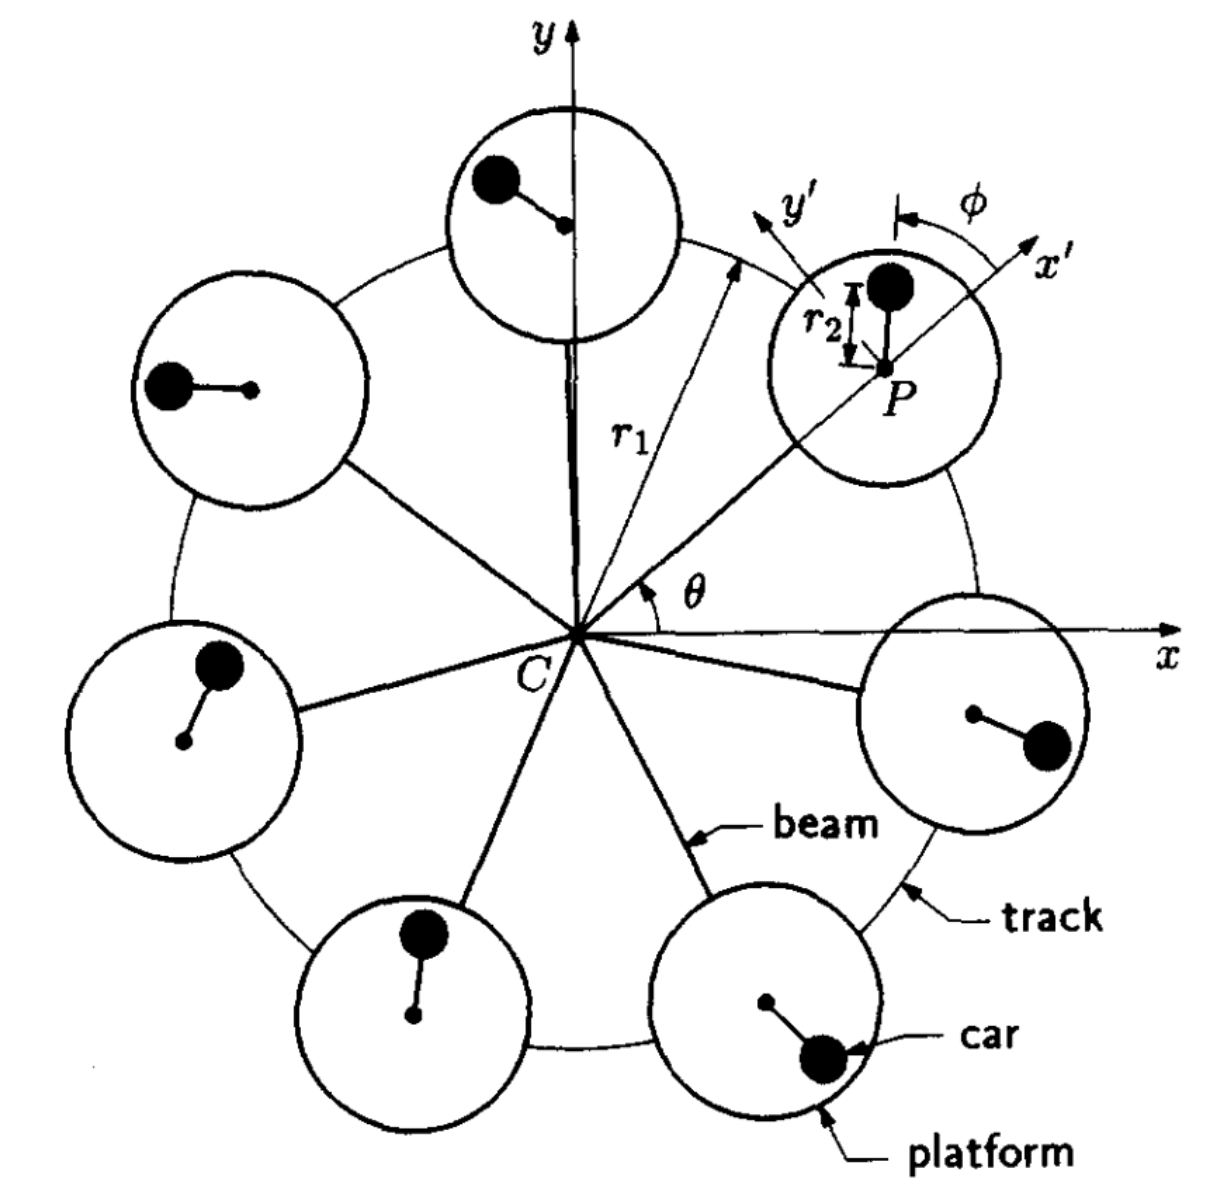
\includegraphics[width=0.5\linewidth]{whirl.png}
  \caption{Plan view of the idealized Tilt-A-Whirl~\cite{doi:10.1119/1.17742}}
  \label{fig:plan_view}
\end{figure}
As can be see, there are $6$ independent parameters in the ODE~\eqref{eq:ode}, 3 of which are our design variables while the rest 3 are fixed. Specifically, the design parameters, $\omega$, $r_2$, and $\alpha_1$, are constrained by their lower and upper bounds: 
  \begin{equation}
  \begin{aligned}
  \frac{\pi}{10} &\le \omega \le \frac{4\pi}{15} \\
  0.1 &\le r_2 \le 1.5 \\
  0 &\le \alpha \le 0.3,
  \end{aligned}
  \end{equation}
while the rest are fixed:
\begin{equation}
\begin{aligned}
r_1 &= 4.3 \\
\alpha_0 &= 0.036 \\
Q_0 &= 20
\end{aligned}
\end{equation}

\section{Mathematical Model}
We start with introducing some notations used in this work. A scalar is denoted as a plain font; bold fonts indicate a variable is a vector, and a subscript number is used to denote the entry of the vector; \eg, $\bm{p}_i$ is the $i$th component of vector $\bm{p}$.

\subsection{Optimization problem}
To use an numerical optimization technique, the physics model in Section~\ref{sec:physics} must be rewritten into a mathematical model. The one used in this work is as follows:
\begin{equation} \label{eq:math_model_1}
\begin{aligned}
max\:\: &\sigma(\frac{\diff\phi}{\diff\tau}) \\
s.t.\:\: &\bm{p}_l \le \bm{p} \le \bm{p}_u\\
         &R(\phi, \bm{p}) = 0
\end{aligned}
\end{equation}
where $\sigma$ ---the standard deviation of $\frac{\diff\phi}{\diff \tau}$--- is the objective function, $\bm{p} = \begin{bmatrix}\omega & r_2 & \alpha_1\end{bmatrix}^T$ is the design variable with lower and upper bounds being $\bm{p}_l$ and $\bm{p}_u$, respectively, and $R(\phi, \bm{p})$ is the ODE~\eqref{eq:ode} which serves as a constraint. 


\section{Analysis model} \label{sec:analysis_tool}
\subsection{Solution to the ODE}
To solve~\eqref{eq:ode} numerically, we first rewrite it into a first-order system:
\begin{equation}\label{eq:1st-order_ode}
\frac{\diff \bm{\psi}}{\diff\tau} = \begin{bmatrix}
F(\bm{\psi}) \\ \bm{\psi}_1
\end{bmatrix}
\end{equation}
where
\begin{equation}
\begin{aligned}
\bm{\psi} &= \begin{bmatrix} \frac{\diff\phi}{\diff\tau} & \phi \end{bmatrix}^T \\
F(\bm{\psi}) &= \frac{\diff\bm{\psi}_1}{\diff\tau} + + \frac{\gamma}{Q_0}\bm{\psi}_1 + (\epsilon - \gamma\alpha)\sin{\bm{\psi}_2} + \gamma\beta\cos{\bm{\psi}_2}.
\end{aligned}
\end{equation}
\eqref{eq:1st-order_ode} is then solved using \texttt{ode45}, giving us both $\phi$ and $\frac{\diff\phi}{\diff\tau}$ as functions of $\tau$.
\subsection{Surrogate model -- Gaussian processing}\label{surrogate}
As mentioned, the dynamic system governed by~\eqref{eq:ode} displays chaotic behavior, which prevents the direct employment of the gradient-based optimization methods because the numerical gradients would see significant oscillations and the function would be nonsmooth. To address this problem, we use the Gaussian processing as a surrogate model to replace the original objective function $\sigma$. 

Practically, there are at least 3 factors affecting the behavior the of Gaussian processing:
\begin{itemize}
  \item sampling
  \item covariance function
  \item likelihood function
  \
\end{itemize}
We use the Latin hypercube approach
Specifically, the Gaussian processing is trained with a sample generated by Latin hypercube approach. As for covariance function, we choose the Matern Covariance function. Finally, Gaussian likelihood is used as likelihood function. Note that a maximization/minimization problem is solved to determine the hyperparameters in the likelihood funciton.

\subsection{Optimization}
Since the surrogate function is smooth, we can use a gradient-based method to solve~\eqref{eq:math_model_1}. On the other hand, since the gradient information of the surrogate is usually not available, it is calculated inside \texttt{fmincon} using finite difference methods. The default algorithm, interior-point, is chosen.

\section{Implementation}

Attention is paid to the modularity of the code; that is, each components is almost independent of the others, and hence, can be completely replaced by another implementation or definition. This gives us the portability and reusability to some extend. For example, function \texttt{sampling} which implements the Latin hypercube approach, can be replaced by Monte-Carlo as long as the API remains unchanged.  In this way, the problem is decomposed into the following parts
\begin{itemize}
  \item \texttt{eqn27} defines the ODE
  \item \texttt{objFunc} computes the objective, \ie, the standard deviation, by calling \texttt{ode45} which itself takes \texttt{eqn27} as an input
  \item \texttt{sampling} generates the data for training \texttt{gaussianProcessing}; it takes \texttt{objFunc} as input
  \item \texttt{gaussianProcessing} takes the sampling results and outputs the hyperparameters \textit{hyp} which is used to define \texttt{surrogate}
  \item \texttt{surrogate} is our surrogate model, \ie, the actual objective function
\end{itemize}

Once these components are defined, the remaining work is to build the workflow of the optimization process. For example, the optimization tool, \texttt{fmincon}, takes a function which itself takes only design variables as parameters. This is different from \texttt{gp}. Therefore, we need to define a wrapper functions, \texttt{surrogate} in our case, to fit API of \texttt{fmincon}.

The workflow used in this work is shown in Algorithm~\ref{alg:opt}, and the implementation in Matlab is attached in Appendix~\ref{app:eqn27}$\sim$\ref{app:multirun}. It is noted that in operation 10 and 11 we update the sampling by appending a new sampling around the newly obtained optimizer $\bm{p}^{iter, *}$, rather than just $\bm{p}^{iter, *}$ itself. This will improve the approximation of the surrogate in a subdomain surrounding $\bm{p}^{iter, *}$, which is motivated by the assumption that the final optimizer is close to $\bm{p}^{iter, *}$.


\begin{algorithm}
  
  \caption{Optimization Algorithm with Surrogate}
  \label{alg:opt}
  \SetKwInOut{Input}{Input}
  \SetKwInOut{Output}{Output}
    \textit{iter} $\gets$ 1\;
    \texttt{sampling}\;
    \Input{\textit{sample\_size}} 
    \Output{$\bm{p}^{iter}$, $\sigma^{iter}$}
    \While {\textit{iter} $\le$ \textit{max\_iter}} 
    {
      \texttt{gaussianProcessing} ()\;
      \Input {$\bm{p}^{iter}$, $\sigma^{iter}$}
      \Output {\textit{hyp}}
      \texttt{obj\_func} = @($\bm{p}$) \texttt{surrogate}(\textit{hyp}, $\bm{p}^{iter}$, $\sigma^{iter}$)\;
      call \texttt{fmincon}, get $\bm{p}^{iter,*}$\;
      \eIf{criteria\_satisfied}{break}
      {
        new sampling ($\bm{p}^{iter,new}$, $\sigma^{iter,new}$) of size $0.2*sample\_size$ around $\bm{p}^{iter,*}$\;
        update sampling: $\bm{p}^{iter+1} = \bm{p}^{iter} \cup \bm{p}^{iter,new}$, $\sigma^{iter+1} = \sigma^{iter} \cup \sigma^{iter,new}$
      }
      \textit{iter} $\gets$ \textit{iter} + 1
    }      
\end{algorithm}

\section{Results and discussion}
The initial sample size is set to be $50$; the initial value is set to be $\begin{bmatrix}
13/60*pi & 0.8& 0.058
\end{bmatrix}^T$, which corresponds to a direct objective $1.5274$. Since the algorithm we use is adaptive, the sample size will keep increasing by $10$ individuals for each iteration. 

The convergence history of the objective approximated by the surrogate and the direct objective is plotted in Figure~\ref{fig:con_hist}. We can see that the surrogate objective flattens after significant oscillations in the first 7 iterations. On the other hand, the direct objective does not see comparable oscillations. After 20 iterations, the direct objective improves by around $75\%$ compared with the initial objective, which proves the justification of the current approach. However, even with an adaptive sampling, the difference between the direct objective and the approximate objective fails to significantly reduce. This may be due to the fact that the direct objective is a nonsmooth and chaotic function, and any smooth surrogate models including the Gaussian processing used in this project is inherently not precise.

\begin{figure} [H]
    \centering
    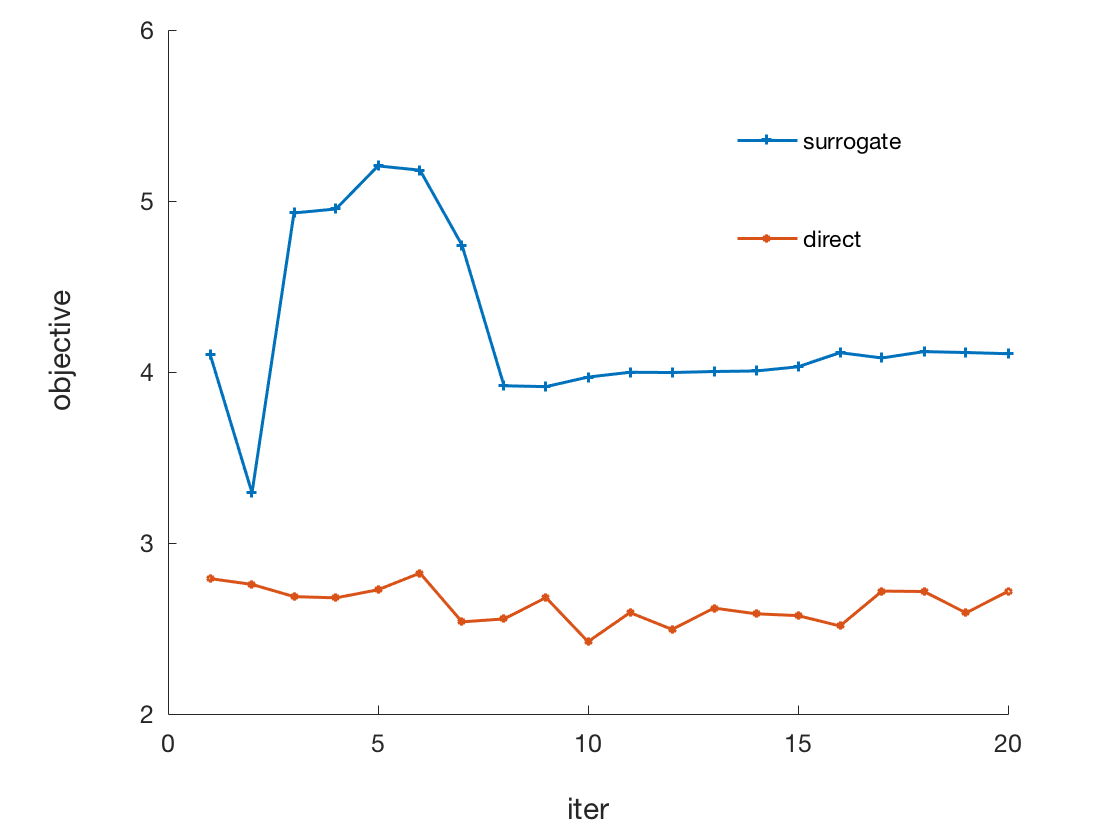
\includegraphics[width=0.75\linewidth]{hist.png}
  \caption{Convergence history of objectives}  
  \label{fig:con_hist}
\end{figure}

\section{Conclusion}
In this work, we use numerical optimization design technique to maximum the Tilt-A-Whirl, a deterministic chaotic system. The Gaussian processing is used as a surrogate model, sampled with the Latin hypercube approach. To improve the performance of the surrogate, we update the sampling in an adaptive way. Although the surrogate is improved little in terms of approaching the direct objective, we do observe an significant improvement in the direct objective value after the optimization.

\bibliographystyle{aiaa}
\bibliography{reference}

\small
\begin{appendices} 
\section{eqn27.m}\label{app:eqn27}
\begin{lstlisting}[language=Matlab]
function dydt = eqn27( tau, y, omega, r2, alpha1 )
% Reference: 
% Chaos at the amusement park: Dynamics of the Tilt?A?Whirl
% by R. L. Kautz.

%  Given parameters
Q0 = 20;
alpha0 = 0.036;
r1 = 4.3;
g = 9.8;
% derived parameters
% tau = 3 * omega * t;
gamma = 1 / (3*omega) * sqrt(g/r2);
eps = r1 / (9*r2);
alpha = alpha0 - alpha1 * cos(tau);
beta = 3 * alpha1 * sin(tau);
% rhs of ode
c1 = -gamma / Q0;
c2 = -(eps - gamma*gamma * alpha);
c3 = - gamma*gamma * beta;
dydt = [y(2); c1*y(2) + c2*sin(y(1)) + c3*cos(y(1))];


\end{lstlisting}

\section{objFunc.m}\label{app:calcobj}
\begin{lstlisting}[language=Matlab]
function [ obj ] = objFunc( x )
omega  = x(1);
r2     = x(2);
alpha1 = x(3);
my_ode = @(t, y) eqn27(t, y, omega, r2, alpha1);
T1 = 0.0;
T2 = 1000.0;
% nSteps = 1000;
% t = linspace(T1, T2, nSteps+1)';
y1_0 = 0.0;
y2_0 = 0.0;
[~, y] = ode45(my_ode, [0, 50], [y1_0; y2_0]);
y0 = y(end, :);
[t, y] = ode45(my_ode, [T1, T2], y0);

% the average
dT = T2 - T1;
y2 = y(:, 2);
y2_avg = mean(y2); % trapz(t, y2) / dT;
deviation = trapz(t, (y2 - y2_avg).^2) / dT;
deviation = sqrt(deviation);
obj = -3*omega * deviation;
end
\end{lstlisting}

\section{sampling.m}\label{app:sampling}
\begin{lstlisting}[language=Matlab]
function [ var, f ] = sampling( sample_size, lb, ub, func )
if size(lb, 2) ~= size(ub, 2)
  error('size(lb, 1) ~= size(ub, 1)');
end
nvar = size(lb, 2);
if nvar == 0
  error('number of variable is zero!')
end
% sampling using Latin hypercube
x = lhsdesign(sample_size, nvar);
% convert from [0, 1] to [lb, ub]
var = zeros(sample_size, nvar);
for i = 1 : nvar
  h = ub(i) - lb(i);
  var(:, i) = lb(i) + x(:,i) * h; 
end
% compute function value
f = zeros(sample_size, 1);
for i = 1 : sample_size
  f(i) = func(x(i, :));
end
end
\end{lstlisting}

\section{gaussianProcessing.m}\label{app:gp}
\begin{lstlisting}[language=Matlab]
function [hyp] = gaussianProcessing(x, y)
% this is needed if you are not running 
% in the Libraries root directory
mydir = '~/Downloads/gpml-matlab-v4.0/';
addpath(mydir(1:end-1))
addpath([mydir,'cov'])
addpath([mydir,'doc'])
addpath([mydir,'inf'])
addpath([mydir,'lik'])
addpath([mydir,'mean'])
addpath([mydir,'prior'])
addpath([mydir,'util'])

% set the squared exponential covariance function
covfunc = {@covMaterniso, 1};
% first component is log(l) and second is log(sigma)
hyp.cov = [log(1/4); log(1.0)]; 

% set the likelihood function to Gaussian
likfunc = @likGauss;
sn = 0.05; %1e-16; % this is the noise level
hyp.lik = log(sn);

% maximize the likelihood function to find the hyperparameters
hyp = minimize(hyp, @gp, -100, @infExact, [], covfunc, likfunc, x, y);
end
\end{lstlisting}

\section{surrogate.m}\label{app:nonlcon}
\begin{lstlisting}[language=Matlab]
function [ f ] = surrogate(hyp, x, f, z)
covfunc = {@covMaterniso, 1};
likfunc = @likGauss;
m = gp(hyp, @infExact, [], covfunc, likfunc, x, f, z);
f = m(1);
end
\end{lstlisting}

\section{run\_opt.m}
\begin{lstlisting}[language=Matlab]
function [a, fmin] = run_opt(x, f)
% initial value, lower and upper bounds
x0 = [13/60*pi; 0.8; 0.058];
lb = [pi/10, 0.1, 0];
ub = [4*pi/15, 1.5, 0.3];

% gaussian processing
fprintf('Gaussian processing...\n');
hyp = gaussianProcessing(x, f);
obj_gp = @(z) surrogate(hyp, x, f, z);

% optimization options
fprintf('Optimizing with surrogate function...\n')
options = optimoptions('fmincon', 'Display','iter', 'MaxIter', 150);
problem.options = options;
problem.solver = 'fmincon';
problem.objective = obj_gp;
problem.Aineq = [];
problem.bineq = [];
problem.lb = lb;
problem.ub = ub;
problem.x0 = x0;

% run fmincon
[a, fmin] = fmincon(problem);
end
\end{lstlisting}

\section{getGeomConstraints.m}\label{app:multirun}
\begin{lstlisting}[language=Matlab]
% lower and upper bounds
lb = [pi/10, 0.1, 0];
ub = [4*pi/15, 1.5, 0.3];
box = ub - lb;

% initial sampling
fprintf('initial sampling...\n');
sample_size = 50;
[x, f] = sampling(sample_size, lb, ub, @objFunc);

% try multiple runs
n_runs = 20;
f_gp = zeros(n_runs);
f_ex = zeros(n_runs);
a = zeros(3, 1);
tol_1 = 1.e-3;
tol_2 = 1.e-3;
fold = 1.0e10;
for i = 1 : n_runs
  fprintf('opt_run = %i\n', i);
  [a, f_gp(i)] = run_opt(x, f);
  f_ex(i) = objFunc(a);
  fprintf('fe = %d, fgp = %i\n', f_ex(i), f_gp(i));

  if abs(f_ex(i) - fold) < tol_1 && abs(f_ex(i) - f_gp(i)) < tol_2
    break;
  end
  fold = f_gp(i);
  lb_i = a - 0.2*box;
  ub_i = a + 0.2*box;
  lb_i = min(lb_i, lb);
  ub_i = max(ub_i, ub);
  [x_i, f_i] = sampling(sample_size*0.2, lb_i, ub_i, @objFunc);  
  x = [x; x_i];
  f = [f; f_i];
  %     x = [x; a'];
  %     f = [f; fobj];
end

iter = (1 : 1 : n_runs);
plot(iter, -f_gp);
hold on;
plot(iter, -f_ex);
hold off;
\end{lstlisting}


\end{appendices}
\end{document}

